\documentclass{article}
\usepackage[margin=1in]{geometry}\usepackage{graphicx,amsmath}
\title{Periodic Pulse: Peak Envelopes and Localization}\author{}\date{}
\begin{document}\maketitle
This report uses the available submitted diagnostics. Upper and lower curves are shape-preserving cubic interpolants through the maximum and minimum in successive 12-unit propagation intervals (approximately one fitted base oscillation period). They describe slow modulation and are not confidence intervals or guaranteed upper and lower bounds. Endpoint traces stop at the first and last selected extrema; no extrapolation is performed. Grey regions have no computed data.
\begin{center}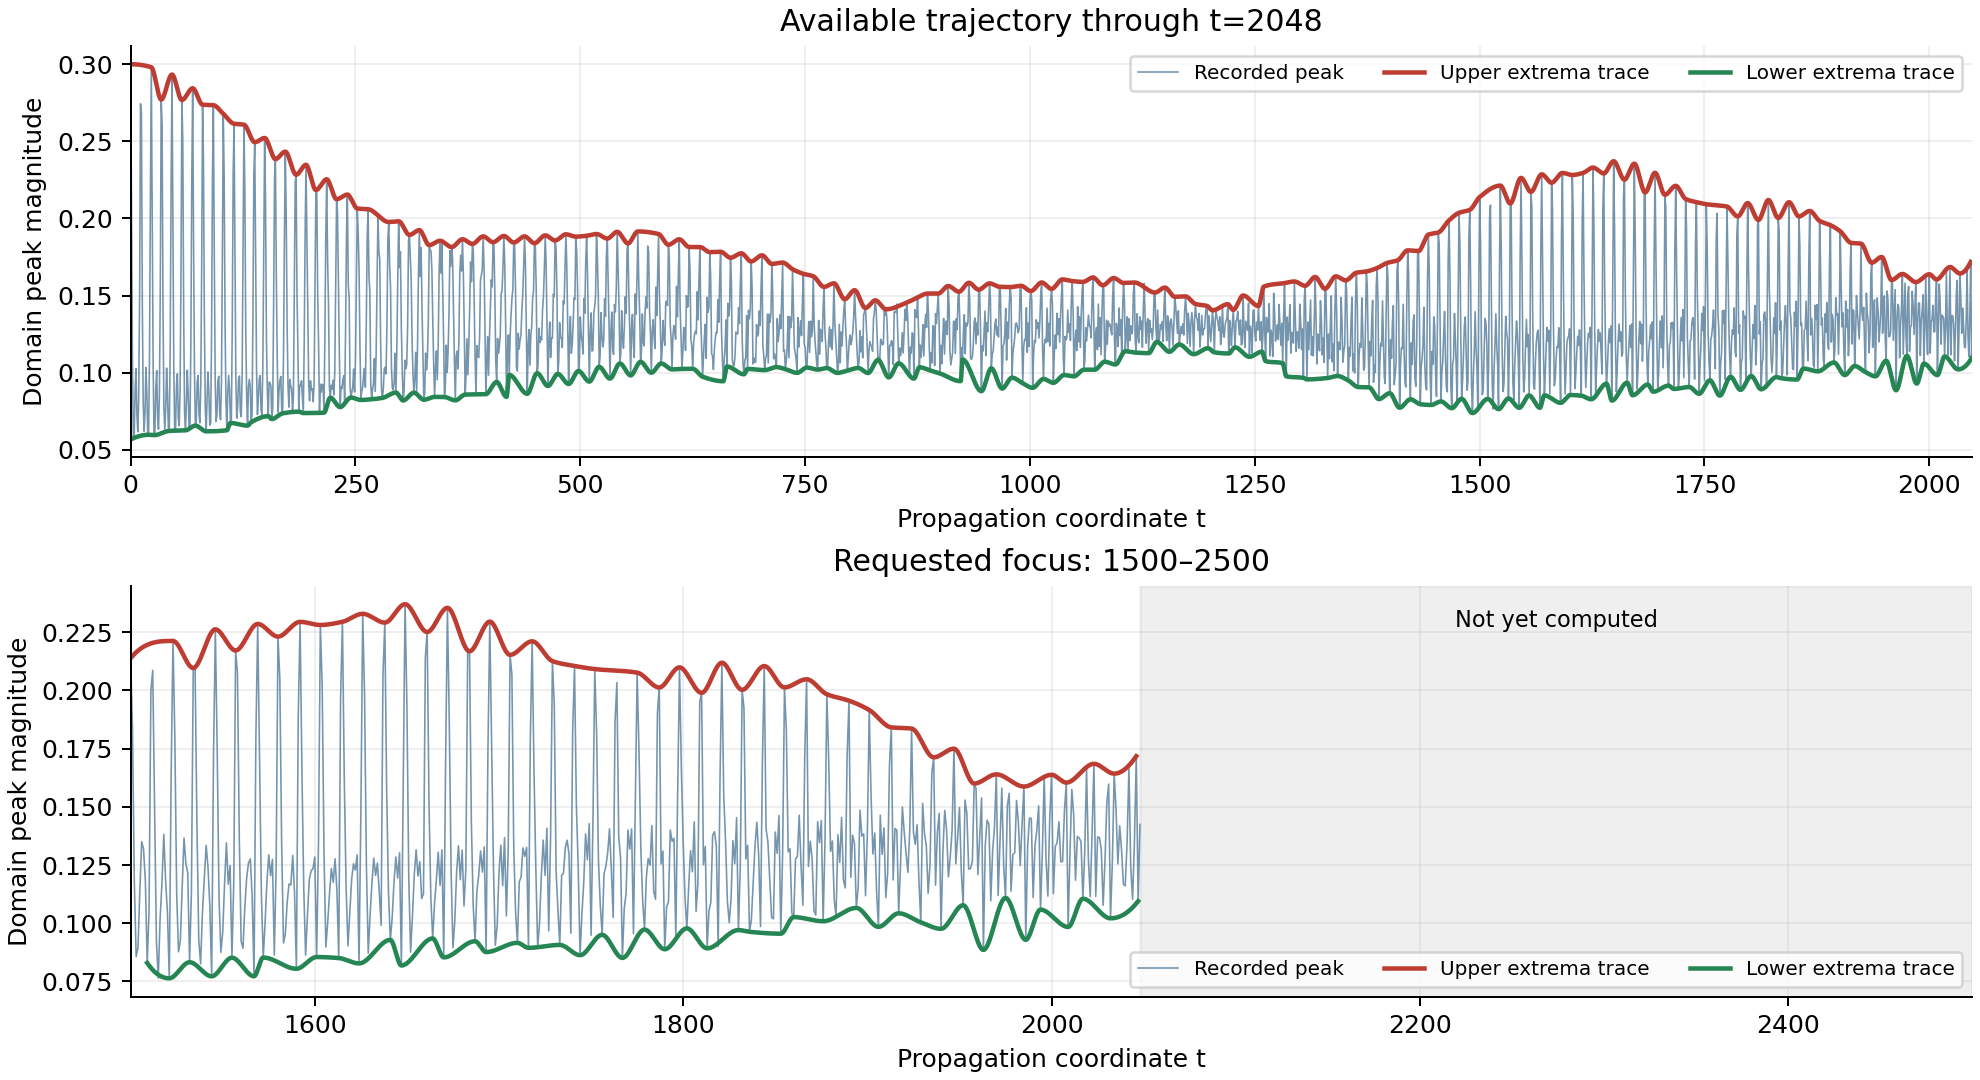
\includegraphics[width=\linewidth]{peak_envelopes.png}\end{center}
\end{document}